\section{Background Information}
The proceeding section attempts to provide background information for this paper.

\subsection{Distributed Systems}
At its core, blockchains are decentralised, distributed systems.
A distributed system is a computing paradigm whereby multiple nodes work together in coordination to achieve a common goal. \cite{bashir_mastering_2017}

\cite{baran_distributed_1964} introduced distributed networks, using a new concept in which computers are connected to other stations rather than switching points like in a centralised system.

Distributed systems are defined as a system in which hardhware or software components located at networked computers communicatte and coordinate their actions via message passing. \cite{coulouris_distributed_2011}

As stated in \cite{coulouris_distributed_2011}, a distributed system must accommodate heterogeneous hardware, operating systems and networks. The networks may differ widely in performance. Systems of widely differing scales, ranging from tens of computers to millions of computers, must be supported.

Replication is key to the effectiveness of distributed systems, it can provide enhanced performance, fault tolerance and high availability. \cite{coulouris_distributed_2011}

nodes in distributed systems can be honest, faulty or mailcious. \cite{bashir_mastering_2017}
\cite{coulouris_distributed_2011} defines arbitrary failures as follows. The term arbitrary or Byzantine failure is used to describe the worst possible failure semantics, in which any type of error may occur. 
For example, a process may set wrong values in its data items, or it may return a wrong value in response to an invocation.

In \cite{lamport_byzantine_1982} the thought experiment of The Byzantine Generals Problem was proposed. 
The scenerio depicts a group of army generals, leading different parts of the Byzantine army plan to attack or retreat from a city. 
The generals can only communicate with eachother via messenger. Communication is necessary in agreeing on a strategy to avoid failure. 
The problem being that one or more of the generals may be traitorous and is attempting to prevent the others from reaching an agreement. 
This necessitates a viable mechanism that enables agreement between actors in the presence of traitors. 
Analogously, distributed systems require agreement amongst nodes, whilst using a channel for communication, even in the presence of Byzantine nodes. This is known as the consensus problem. \cite{fischer_consensus_1983}
The consensus problem occurs when attempting to achieve reliability in a distributed system, in the presence of faulty processes. 
A system requires processes to reach an \emph agreement on a value after one or more processes propose what the value should be. 
In a system such that: each process $p_i$ communicates with other processes via message passing (assuming communication is reliable), up to some number $f$ of the $N$ processes are faulty, the remainder of processes are correct.\linebreak[1]
Reaching consensus is achieved as follows. 
Every process $ p_i $ starts in an \emph{undecided} state and \emph{proposes} a single value $v_i$.
The processes communicate with eachother and exchange values. 
Each process then sets the value of a \emph{decision variable}, $d_i$. 
In doing so the process enters the \emph{decided} state and can no longer change $d_i$.\cite{coulouris_distributed_2011}
\begin{enumerate}
	\item Termination: Eventually each correct process sets a decision variable.
	\item Agreement: The decision of all correct processes is the same.
	\item Integrity: If the correct processes al proposed the same value, then any correct process in the \emph{decided} state has chosen that value.\cite{coulouris_distributed_2011}
\end{enumerate}

The Byzantine Generals Problem was solved in \cite{castro_practical_1999}, where the Practical Byzantine Fault Tolerance (PBFT) algorithm was introduced.

The first practical implementation of PBFT was produced with the inception of Bitcoin, in which the Proof-of-Work (PoW) algorithm was developed as a consensus mechanism. \cite{nakamoto_bitcoin_2019}

In \cite{ongaro_search_2014}, Raft was introduced as a consensus algorithm, which produced similar results to and was as efficient as Paxos - a family of protocols for solving consensus, presented in \cite{pease_reaching_1980}.
Raft was a successful attempt at restructuring a consensus mechanism in order to enhance understandability. Raft is crash fault tolerant, but lacks in Byzantine fault tolerance. \cite{ongaro_search_2014} 




\subsection{Hyperledger Fabric}

Hyperledger Fabric's key design features, as introduced in \cite{androulaki_hyperledger_2018}, are explored next.
A channel, in Hyperledger Fabric, is a private "subnet" for communication between multiple organisations on the network \cite{noauthor_channels_nodate}. 
Assets, defined by chaincode, are exchanged across the network. These are stored as a collection of key-value pairs, represented in binary and/or JSON, with state changes recorded as transaction on a channel ledger. 
Chaincode is Hyperlegder Fabric's version of smart contracts. Chaincode is a program, which can be written in general-programming languages Go, JavaScript (for Nodejs runtime) or Java, that implements a prescribed interface.

Chaincode, the software defining assets, also defines the transaction instructions for manipulating the assets; chaincode is the business logic. Invocation of chaincode is recorded in a ledger.
Ledgers serve as a sequenced, tamper-proof record of all state transitions which are a result of transactions \cite{noauthor_ledger_nodate}.
Ledgers are comprised of a blockchain "chain" to store the records in blocks and a state database \cite{noauthor_hyperledger_nodate}. 
The chain is transaction log, structured as hash-linked blocks where each block contains a sequence of $N$ transactions \cite{noauthor_hyperledger_nodate}.
Channels are used to communicate privately between organisations, enabling privacy.
Each channel contains a ledger, for that channel, peers also maintain a copy of the ledger for each channel of which they participate. This is used to maintain consistency across peers. 

Hyperledger projects follow a design philosophy, which includes a modular, extinsible approach; enabling interoperability.
Design puts an emphasis on secure solutions, crucial to systems using sensitive data.
Hyperledger's token-agnostic approach simplifies bringing blockchain to business infrastructure. \cite{noauthor_hyperledger_2017}

Hyperledger projects embrace security by design and follow the best practices specified by the Linux Foundation's Core Infrastructure initiative \cite{noauthor_hyperledger_2017}. \footnote{https://www.coreinfrastructure.org/}

As discussed in \cite{androulaki_hyperledger_2018}, blockchain systems typically, both permissioned and permissionless, follow the order-execute architecture. 
This execution style involves ordering transactions first, using a consensus protocol, then executes them in the same order on all peers sequentially.\footnote{This report follows the convention set in the Hyperledger Fabric whitepaper; naming the transaction execution (named "transaction validation" in blockchains such as Bitcoin \cite{nakamoto_bitcoin_2019}) \emph{transaction execution} to bring the terminology together.}
\begin{figure}[H]
  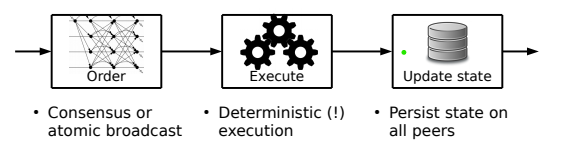
\includegraphics[scale=0.9]{order-execute}
  \caption{Order-execute architecture in replicated services}
  \source{\cite{androulaki_hyperledger_2018}}
\end{figure}

Whilst the order-execute architecture is conceptually simple and therefore widely used, there are drawbacks which occur when using it for a general-purpose permissioned blockchain.\cite{androulaki_hyperledger_2018}
The most significant disadvantages are as follows: 
\emph{Sequential execution}. Executing transactions sequentially on all peers limits the effective throughput that can be achieved on the blockchain \cite{androulaki_hyperledger_2018}.
One solution to this problem, used by Ethereum \cite{wood_ethereum_nodate}, utilises the concept of \emph{gas} consumed by a transaction execution, which is converted at a \emph{gas price} to a cost in the cryptocurrency and billed to the transaction submitter.
This solution is excellent for use in permissionless blockchains, though does not suffice when designing a general-purpose, permissioned, token-agnostic, blockchain like Hyperledger Fabric \cite{androulaki_hyperledger_2018}.

In Hyperledger business blockchain frameworks consensus is reached by performing two seperate activities:
\begin{enumerate}
  \item Ordering of transactions
  \item Validating transactions
\end{enumerate}
In the first step, the transactions are received from the client.
An ordering service is used to order the transactions. 
To enable confidentiality, the ordering service may be agnostic to the transaction; that is, the transaction content can be hashed or encrypted.\cite{noauthor_hyperledger_2017}
This is extremely benificial to this system, as maintaining confidentiality is essential to abiding by the GDPR \cite{noauthor_general_nodate}.

Consensus in Hyperledger Fabric is further broken into 3 phases: \emph{Endorsement}, \emph{Ordering} and \emph{Validation}.
\begin{enumerate}
  \item Endorsement is driven by policy (eg. m of n signatures) upon which participants endorse a transaction. 
  \item Ordering phase accepts the endorsed transactions and agrees to the order to be committed to the ledger.
  \item Validation takes a block of ordered transactions and validates the correctness of the results, including checking endorsement policy and double-spending.
\end{enumerate}

Hyperledger Fabric distributed applications consist of two parts: A smart contract, called \emph{chaincode}, which is program code that implements the application logic and runs during the \emph{execution phase}.
As well as an \emph{endorsment policy} that is evaluated in the \emph{validation phase}.
Endoresement only requires a subset of peers, this enables parallel execution and eliminates any non-determinism, as inconsistent results are filtered out before ordering.
Because non-determinism has been eliminated, Fabric is the first blockchain technology that enables use of standard programming languages. \cite{androulaki_hyperledger_2018}
This proves useful in systems such as this, as adoption is easiest when current technologies can be used instead of domain-specific languages, like Solidity for the Ethereum blockchain \cite{noauthor_ethereum_nodate}.

The proposed system is utilising v2.3.2, at the time of writing, the latest release of Fabric. \ref{appendix:version}
Fabric v2.0 delivers important new features and changes for users and operators. % Support for new application and privacy patterns, enhanced governance around smart contracts, and new options for operating nodes. 
Namely, the addition of decentralised governance for smart contracts. 
A new implementation of the chaincode lifecycle allows multiple organisations to agree on parameters of chaincode, before it can be used to interact with the ledger. 
These parameters include: the chaincode package name, version, and endoresement policy \cite{noauthor_whats_nodate}.
Version 2.3 removed the requirement for a system channel when creating a channel, simplifying the administration process. \cite{noauthor_create_nodate}

In Fabric, to participate, every node and user that interacts with a network needs to be part of an organisation. \cite{noauthor_using_nodate}

Members of a network in Fabric enroll through a trusted Membership Service Provider (MSP). \cite{noauthor_introduction_nodate}
An MSP serves as a trusted authority, that is in control of the governing of identities for its organisation. 

An MSP is a structure of folders added to the network configuration, to define the permissions and roles in an organisation. 
Certificate Authorities (CAs) generate the certificates that represent identities, the MSP is where these reside. 
Roles in organisations are assigned to the identities, by the MSP. 
MSPs also hold a copy of the revoked certificates, for the organisation, which is checked whenever the certificate is attempting to be used. \cite{noauthor_membership_nodate}
This list is called a Certificate Revocation List (CRL) \cite{cooper_internet_nodate} and is stored by the issuing CA. \cite{noauthor_identity_nodate}
MSPs come in two flavors, \emph{local MSPs} have a scope limited to the organisation they are part of and reside on the organisation's node. Every node requires an MSP.
\emph{Channel MSPs} define administrative and participatory rights at a channel level. These channel MSPs include the MSPs of the organisations on the channel, enabling the control of relationships between the channel participants. \cite{noauthor_membership_nodate}

Fabric CA is the default Certificate Authority in a Fabric network. Acting as a root CA, Fabric CA issues the certificates required for the MSPs to implement identities and roles. \cite{noauthor_identity_nodate}

\section{System Design}

The following section will detail the design of the proposed system.
Using the C4 model for visualing software \cite{noauthor_c4_nodate}, diagrams shall be generated for visualisation of the system \ref{appendix:c4plantuml}.
The C4 model employs an "abstraction-first" approach to diagramming architecture \cite{noauthor_c4_nodate}. 

The system proposed in this paper is that of an Immunisation-Information-System (IIS), which utilises blockchain to supply a reliable and tamper-proof collection of Immunisation records. 

Though medical records have evolved into electronic records, the immunisation systems around the globe have not evolved \cite{abbas_review_2014}.

Evolving these systems is a necessity for the international community to posses a fair, transparant and safe IIS, with the capabilities for citizens access to their records as well as an avenue of confirming them for those who need the verification.

Hyperledger Fabric has been chosen as the framework to build this system. 
Because, as discussed in \cite{yu_comparison_2020}, Hyperledger Fabric brings fine-grained control to applications which is suitable for the healthcare industry.

The proposed Distributed-Immunisation-Information-System (DIIS) shall be comprised of both a web application and a Hyperledger Fabric network. 
The web application will facilitate communication from users to the underlying blockchain network.

Hyperledger Fabric enables organisations to collaborate in forming, running and utilising blockchain networks \cite{noauthor_blockchain_nodate}.

The main users using the web application will be those performing administrative processes - employees of health authorities, which are acting as the organisations. 

The web application shall also enable citizens access to their immunisation records, that will be entered by the health authority in the citizen's nation.

To ensure all records are that of fully vaccinated patients, entering the immunisation record information should be done after all required doses are administered. 

If this requirement is followed correctly, all records in the system will be that of fully vaccinated patients. 

The system shall not provide any assistance in managing records for patients who have had the first of multiple doses etc.

Additionally, immunisation verifiers, such as border agents, school administrators, venue admissions staff will be able to lookup a citizen's provided universally unique identifier (UUID) to confirm their status of immunisation.

\begin{figure}[H]
    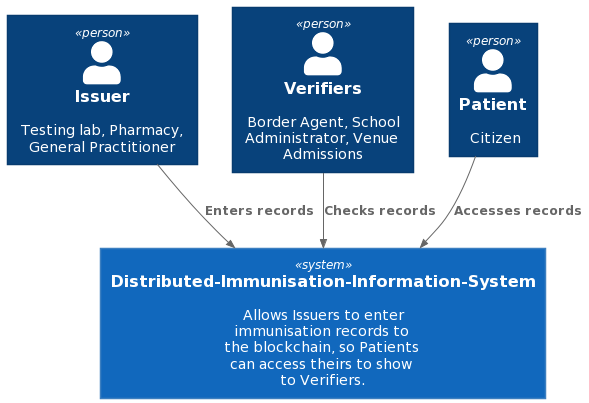
\includegraphics[scale=0.5]{system-context}
    \caption{System context diagram for DIIS}
    \label{fig:context}
    \source{\cite{androulaki_hyperledger_2018}}
  \end{figure}

Figure \ref{fig:context} provides visual context to the system. As shown, immunisation record issuers are those who administer immunisations to patients. 
Issuers will enter the information of the immunisation record into the system, allowing patients constant access to their records. 
Verifiers, those who need verification of immunisation from citizens, shall be able to lookup information via credentials provided by citizens. 
This enables autonomy over a person's records. 

Using Hyperledger Fabric maximises the potential for interoperability of Electronic Health Record (EHR) systems across borders, as it reduces the requirement for particular infrastructure. 
Discussed in \cite{kierkegaard_electronic_2011}, this is important to the EU as displayed in \cite{noauthor_directive_2011}. 
Maintaining this requirement is key for adoption of the system by EU nations.

A web application will facilitate communication with the underlying Fabric network. 
Organisations will have the option to develop their own applications, enabled by the nature of Open-source software. 
However, considerations have been made in selecting the default application SDK as the correct choice could simplify adoption. 
The default application will be built using the Hyperledger Fabric Nodejs SDK \ref{appendix:nodesdk}. 
This decision is the result of the desire to maintain a flexible system, through ensuring the minimal requirements for adoption. 
Nodejs possesses the advantage in terms of ease of use, when compared to the other available SDKs such as Java and Go, as it enables the utilisation of JavaScript for both client and server-side scripting \cite{nodejs_documentation_nodate}. 
Also, Fabric has a Performance Traffic Engine tool (PTE), specific to Node \ref{appendix:pte}. 
Opting for the Node SDK enables the use of the PTE in testing the network. 

\subsection{Application}

\begin{figure}[H]
  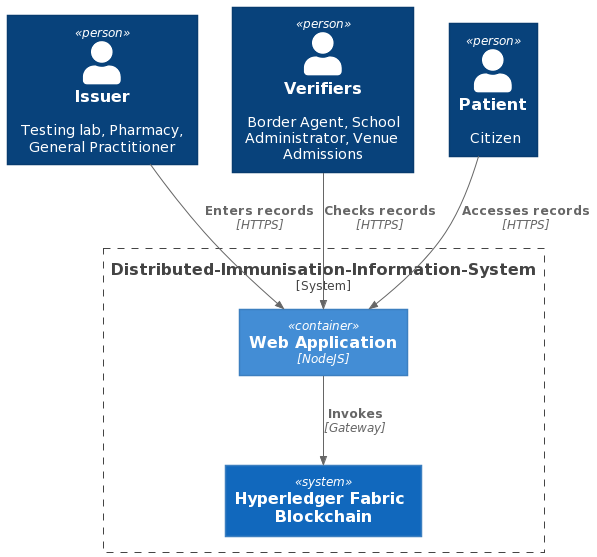
\includegraphics[scale=0.5]{system-lower-view}
  \caption{A lower-level system view}
  \label{fig:lower}
\end{figure}

Figure \ref{fig:lower} shows a lower-level view of the proposed system, including the web application. 
This serves as a better picture to how this system communicates with the underlying blockchain network. 
All users will make use of the application as a means of either entering records, accessing records or validation of records. 
The web application takes advantage of a gateway to handle the interactions between the application and Fabric network \ref{appendix:fabnetgate}. 
A gateway is setup on the server-side of the application and uses a user's identity, stored in a wallet, to sign transactions \cite{noauthor_gateway_nodate}. 
Fabric has two types of gateway, static and dynamic. 
The latter shall be utilised in this application. This enables service discovery by the gateway, allowing it to find all connected peers and orderers within the network using the gossip protocol; Fabric's data dissemination protocol, which broadcasts information to and from peers in a channel \cite{noauthor_gateway_nodate}. 



\begin{figure}[H]
  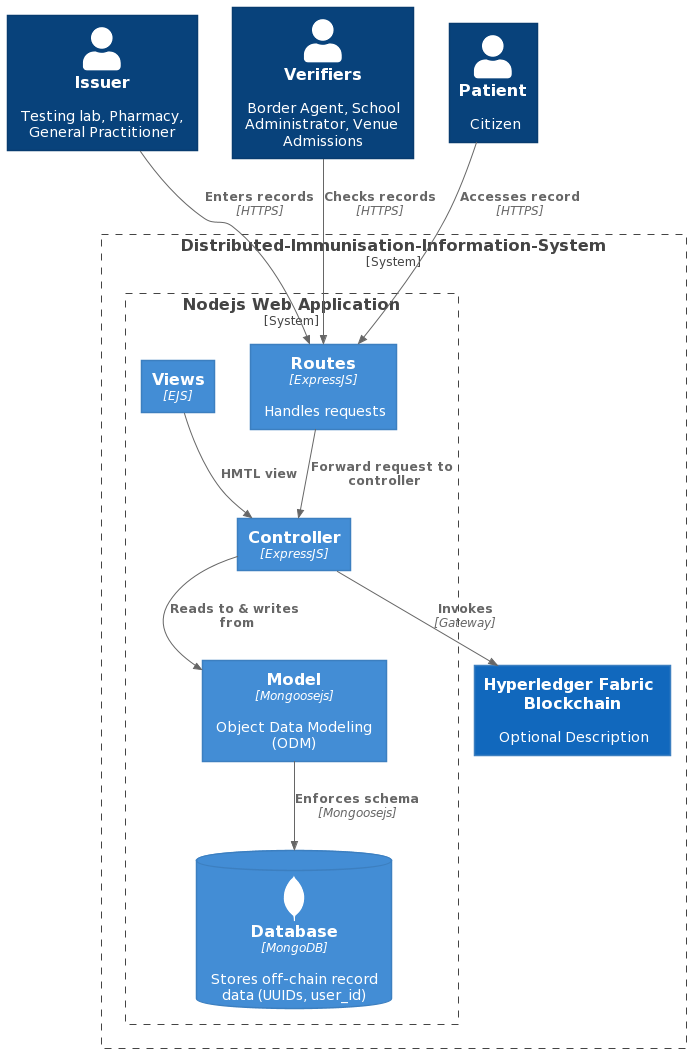
\includegraphics[scale=0.5]{lower-lower}
  \caption{Component diagram for the DIIS}
  \label{fig:lower-lower}
\end{figure}

In figure \ref{fig:lower-lower} a component-level diagram is displayed, to show how the containers in figure \ref{fig:lower} are constructed. 
Design of the web application used to communicate with the Fabric network has been achieved using the Model-View-Controller (MVC) architecture. 
The web application is seperated into three main components, each built to handle specific tasks. 
This is to maintain a seperation of concerns \cite{richards_software_2015}.
Designing this way ensures modularity \cite{laplante_what_2007}.
Encapsulation of components is essential to ensuring minimal system-breaking bugs, that may occur when code is changed, through added flexibility \cite{leff_web_application_2001}.
It also aids in keeping the system as infrastructure agnostic as possible.
ExpressJS is the framework of choice, for building with Nodejs. 
It provides middleware that aids backend functionality by providing handling of routes, requests and views \cite{noauthor_express_nodate}.
An array of template engines are available to use with Express, a selection has been made for this system to use EJS.
EJS provides embedded JavaScript template functionality, using plain JavaScript enables speedy execution and simple debugging \cite{noauthor_ejs_nodate}.

MongoDB will be used as a document-based database, enabling the use of JSON (JavaScript Object Notation \cite{noauthor_json_nodate}) to model data. 
Documents are stored in BSON (Binary JSON), which enables faster parsing \cite{noauthor_json_bson_nodate}. 
Mongoose, an Object Data Modelling (ODM) library for MongoDB, will be used to model application data in Nodejs. Mongoose provides built-in validation and query building. \cite{noauthor_mongoose_nodate} 

Application will be containerised using Docker, building containers both for the application and database. 
Docker Compose allows the user to specify dependencies between services using the \lstinline{depends_on} command \cite{noauthor_compose_2021}. 
This command shall be used to ensure the Nodejs container waits until the database container is "healthy" using a \lstinline{healthcheck} \cite{noauthor_compose_2021}.

Credentials for patients shall be provided in the form of a UUID (Universally Unique IDentifier), defined in \cite{noauthor_rfc4122_nodate}.
UUIDs will be created using a package for Node \ref{appendix:uuid}. 
Using an encrypted email service to give patients their credentials for use in the application was debated, as the NHS already utilises this \cite{noauthor_guidance_nodate}. 
However, for the system to remain as infrastructure agnostic as possible, the credentials shall be received by patients in-person when the immunisation is administered.

\subsection{Network}
This section will explore, in detail, the backbone of the system; the Hyperledger Fabric blockchain network. 
The intial network for the system is based on the Fabric test network, provided in the official documentation for Hyperledger Fabric \cite{noauthor_using_nodate}, contained in the "fabric-samples" repository \ref{appendix:testnet}.
It is kept to a limited configuration for ease of development:
\begin{enumerate}
\item{It includes two peer organizations and an ordering organization.}
\item{For simplicity, a single node Raft ordering service is configured. Though, when in production the ordering nodes may also be implemented by those organisations that wish to bypass relying on a central admin managing nodes.}
\item{A TLS Certificate Authority (CA) is deployed, for use with user identities.}
\end{enumerate}

A central, trusted authority, such as the World Health Organisation (WHO) shall maintain the ordering organisation. \footnote{https://www.who.int/}

Each organisation in the network has control over its members, through Fabric's MSPs. 
This control also extends to the organisation's data, this shall not be shared with other organisations unless allowed by the organisation. 
Private channel capabilities ensure that data will only be shared with those authorised by the owning organisation. 

\begin{figure}[H]
  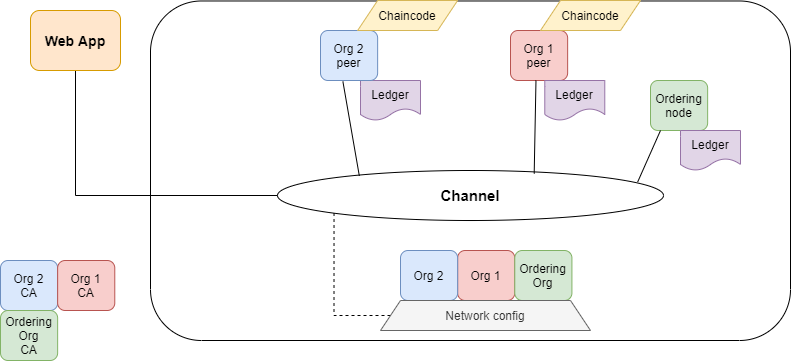
\includegraphics[scale=0.5]{network-diagram}
  \caption{Diagram of the underlying blockchain network}
  \label{fig:network-diagram}
  \source{Adapted from \cite{noauthor_how_nodate}}
\end{figure}

Figure \ref{fig:network-diagram} shows the basic setup for the network. 
The organisations have established a network, which necessitates all organisations agreeing on a configuration. 
The configuration defines the roles each organisation plays in the network, more specifically; this is what makes the ordering organisation just that, instead of a participating organisation.

The channel configuration policy is defined in \lstinline{configtx.yaml}, this can be found in the appendices \ref{appendix:configtx}. 
Firstly, organisations are defined. With each definition for an organisation a default policy is also defined. 
Each policy has a type; either \lstinline{Signature} or \lstinline{ImplicitMeta}. 
\lstinline{Signature} policies establish which type of user must sign for a policy to be satisfied. 
\lstinline{ImplicitMeta} policies are valid only in the context of channel configuration, these policies aggregate the policies defined by \lstinline{Signature} policies. 
The implicity comes from the policy being constructed based on the policies defined in organisation definitions. 
\lstinline{ImplicitMeta} policies are satisfied when all policies aggregated by it are satisfied. \cite{noauthor_policies_nodate}
When defining the orderer organisation for this network, the \lstinline{Signature} policies shall require a member of the orderer organisation's MSP to sign. 
This is achieved using the "Rule" \lstinline{"OR('OrdererMSP.member')"} in the \lstinline{Signature} policy for the orderer organisation. 
When defining the application, policies are also defined. 
Utilising the \lstinline{ImplicitMeta} policy type allows for reference of the sub-policies defined for each organisation \cite{noauthor_policies_nodate}. 
Two important policies defined in the application section are \lstinline{LifecycleEndorsement} and \lstinline{Endorsement}. 
\lstinline{LifecycleEndorsement} governs who needs to approve a definition for chaincode. 
\lstinline{Endorsement} is the default chaincode endorsement policy. 
In this network both policies shall use the rule \lstinline{MAJORITY Endorsement}, ensuring that the majority of peers belonging to the different organisations are required to execute and validate a transaction before the transaction is considered valid \cite{noauthor_policies_nodate}.

Figure \ref{fig:network-diagram} displays the basic setup for the network, including only two organisations for simplicity's sake. 
As shown, each organisation joins peers to the channel, this includes the ordering organisation. 
Each peer node shall contain a copy of the ledger of the channel \cite{noauthor_how_nodate}. 
Excluding the ordering organisation's peer, each peer also holds a state database. 
The state database, stores information on the world state. 
The world state holds the current value of attributes of the assets, this is useful as it negates the need to traverse the blockchain to gather an assets current value. \cite{noauthor_ledger_nodate}
As shown, there will be one application utilised by the organisations to access the underlying network. 
All organisations posses their own CA, which generates the certificates for the nodes, admins and organisation definitions \cite{noauthor_how_nodate}.

\subsection{Chaincode}
The following section will present the design of the chaincode for the system. 
\cite{alexaki_blockchain-based_2018} suggests that medical records should contain metadata of a patient-provider encounter (visit date/time, location, etc.), 
the data shall be stored off-chain and should be entered when the record is produced. 
\cite{dye_covid-19_2021} states that the duration of protection conferred by vaccines should
be tied to expiry dates.
To ensure immunisation records expire, the ledger must store metadata on the particular immunisation records to ensure they can be invalidated when the expiration is reached. 
This will be implemented using a timestamp, created on the client side, in the records stored on-chain. 

Go has been selected as the language for writing chaincode, for this system. 
As discussed in \cite{foschini_hyperledger_2020}, language choice has an impact on the latency of transactions. 
\cite{foschini_hyperledger_2020} found Go to be the best performing language available for writing Hyperledger Fabric chaincode.  

The chaincode for this system will represent "Records", immunisation records, the initial chaincode package will be called "record\_1.0". The implementation of this is documented in subsequent sections. 
Representing the records as chaincode, or smart contracts, enables the manipulation of records by organisations that "own" them. 
The chaincode written for this system can be found in the appendix \ref{appendix:chaincode}. 



\section{Implementation}
The following section will detail the implementation process of the system.

\subsection{Chaincode}
Fabric networks use chaincode to initialise and manage the ledger state, through transactions submitted by applications. \cite{noauthor_writing_nodate}
To use chaincode in a network organisations need to agree to the parameters, the name of the chaincode, version and the endorsement policy. 
\cite{noauthor_writing_nodate} explains that the agreement is reached using the following steps:
\begin{enumerate}
  \item Package the Chaincode
  \item Install the chaincode on peers: Each organisation that will utilise the specific chaincode, to endorse transactions or query ledgers, needs to execute this step.
  \item Approve chaincode definition for organisation: This step also requires completion from each organisation that will use the chaincode. By default, the chaincode needs to be approved by atleast a majority of organisations before it can be deployed on a channel.
  \item Commit the chaincode definition to the channel: After the chaincode is approved by a sufficient number of organisations, one organisation can commit the chaincode definition.
\end{enumerate}

Chaincode needs to be packaged in a tar file for it to be installed onto peers \cite{noauthor_fabric_nodate}. Using the Fabric peer binaries, the following command can be used to skip manually adding the necessary "metadata.json" file which required in the tar file.
\begin{lstlisting}[language=bash, caption={peer lifecycle chaincode package command}]
  # create the chaincode package using the peer lifecycle chaincode package command
  peer lifecycle chaincode package record.tar.gz --path ../asset-transfer-basic/chaincode-go/ --lang golang --label record_1.0
\end{lstlisting}

Though not necessary for Fabric networks, it would be useful for organisations to synchronise their labels for chaincode. 
This will be a standard for adopting this system.

Installation of chaincode on peers can be executed via CLI or an SDK \cite{noauthor_fabric_nodate}. 
This network relies on access via CLI, to install chaincode. 



\begin{figure}[H]
  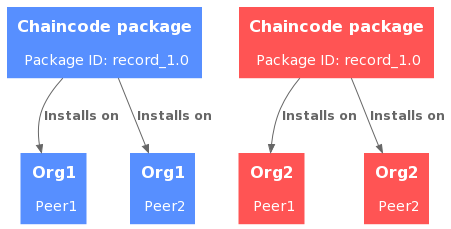
\includegraphics[scale=0.7]{cc-diagram-redo}
  \caption{Peer admin from two organisations installs the chaincode package record\_1.0}
  \source{Adapted from \cite{noauthor_fabric_nodate}}
\end{figure}

In this system is it not necessary to set the endorsement policy for the chaincode as it will be utlising the default value, which requires that a majority of organisations endorse a transaction. \cite{noauthor_fabric_nodate}


\subsection{Web Application}
The following section shall cover the implementation of the web application, of which the design was explored previously. 
Development was aided by the supplied test-application in the documentation for Hyperledger Fabric \ref{appendix:testapp}.
This provided sample, application uses JavaScript to interact with the underlying network via Fabric's Node SDK \ref{appendix:testapp}.

The complete code for the web application can be found in the appendix \ref{appendix:webapp}.

Development of the application was utilising the Fabric test network \ref{appendix:testnet}, provided with the official documentation for testing applications and chaincode.
All that is required to use the test network are the Hyperledger Fabric Docker images and samples. \cite{noauthor_using_nodate}
The topology of the test network has been explored previously. 

JavaScript's "strict mode" is used throughout the application. 
Strict mode ensures cleaner code, by preventing the use of undeclared variables \cite{noauthor_referenceerror_nodate}. 
Strict mode is supported by all modern browsers, except Internet Explorer 9. Though, "use strict" is just a string, so IE 9 will not throw an error even if it does not understand it \cite{noauthor_javascript_nodate}.

\subsubsection{Network Deployment}
The sample test network comes with provided scripts to deploy the network \ref{appendix:testapp}. 

To bring up the network the shell script \lstinline{network.sh} is executed with the command \lstinline{up}. 
A channel also needs creating, as does a CA for the network, so we pass the command \lstinline{createChannel -c mychannel} and the flag \lstinline{-ca}. 
The \lstinline{createChannel} command also ensures the organisations' peers join the created channel \cite{noauthor_using_nodate}.
The full command is \lstinline{./network.sh up createChannel -c mychannel -ca}.
During this step, an admin user for the organisations is boostrapped with the CA.  

Next, the chaincode, of which the implementation was detailed previously, is installed. 
This is performed using, again, the "network.sh" shell script. 
The command \lstinline{deployCC} is passed, with the \lstinline{-ccn} flag to specify the name of the chaincode, which is \lstinline{record}. 
Additionally the \lstinline{-ccp} flag is supplied with the command with the location of the chaincode package \lstinline{../app/chaincode}, as well as the \lstinline{-ccl} flag with the option \lstinline{go} to indicate the language the chaincode was written in. 
The full command used is \lstinline{./network.sh deployCC -ccn record -ccp ../app/chaincode -ccl go}. 
The full logs for process can be found in the appendix \ref{appendix:testnetlogs}.

\subsubsection{Application Details}
Once the test network is running, the application can be deployed. 

lstinline{node app.js} starts the application, from the commandline. 

The MongoDB database is connected at startup, using the \lstinline{db.js} file \ref{appendix:dbjs}. 
First, an object for connection to the database via mongoose is instantiated. 
Connection options, for the database, are setup as constants and then provided in the url passed as a parameter to the \lstinline{mongoose.connect()} function. 

The main file for the app, \lstinline{app.js}, imports necessary objects at the beginning of the file and can be found in the appendix \ref{appendix:appjs}. 
The Express api is imported as an object, \lstinline{express}, this is how an Express application is created. \cite{noauthor_express_nodate}
The Express version used in this application is 4.16.4. 
A router is also imported, this is how Express applications handle how the applications endpoints (URIs) respond to client requests \cite{routing_express_nodate}.
A path for the views is then defined, next a port to open the application via http. 
Next, the template engine, \ref{appendix:ejs}, is defined. 
This application uses EJS to dynamically serve HTML files. 
Using a template engine simplifies passing data to the client view from the backend. 
The app finally listens for connections on the previously defined port. 

\paragraph{Routes}
A folder named \lstinline{routes} contains two files dictating the routes for the application. 
\lstinline{index.js}, found in appendix \ref{appendix:indexroute}, imports a router object from Express and defines the index route. 
The script then sends the \lstinline{index.html} file as a client view.
The module is then exported as \lstinline{router}. 
The file \lstinline{records.js}, found in appendix \ref{appendix:recordroute}, also imports the router object and exports the module as \lstinline{router}. 
This file defines routes necessary for \lstinline{GET} and \lstinline{POST} requests used to add records, generate UUIDs, check records and serve an index page for the record manipulation functionality. 
These routes are responsible for calling the functions, dependant on which request is sent, defined in \lstinline{records.js} \ref{appendix:controller} - the file is located in the controller directory. 

\paragraph{Controller}
The file \lstinline{records.js} represents the controller for the application. 
Imports are made at the top of the file, notable imports follow. 
\lstinline{Record} model is imported in the form of an object, for use by the controller to structure data. 
A package for generating UUIDs \ref{appendix:uuid}. 
The \lstinline{Gateway} and \lstinline{Wallets} classes are imported from \lstinline{'fabric-network'}, information on these can be found in the appendices; \ref{appendix:fabnetgate}, \ref{appendix:fabnetwallets}. 
\lstinline{FabricCAServices} is an API, imported from \lstinline{'fabric-ca-client'} \ref{appendix:nodeca}, enabling CA functionality. 
\subparagraph{Controller utility files}
Utility files, provided with the Hyperledger Fabric test application, have been utilised in the controller \ref{appendix:utils}.
The file \lstinline{CAUtil.js} provides functions for building a CA client, enrolling the admin user and registering as well as enrolling users. 
The function \lstinline{registerAndEnrollUser()} first checks if the user is already enrolled, next uses an admin user to build a user object for authentication with the CA, then registers and enrolls the user.
An admin account, bootstrapped with the \lstinline{nettwork.sh up} script, is used as the registrar for the CA.
\lstinline{enrollAdmin()} is a function that, when called, generates, locally, a private key, public key, and X.509 certificate for the admin.
As the admin account was bootstrapped at startup, the admin only needs to be enrolled.
Using a Certificate Signing Request, described in \cite{noauthor_rfc2986_nodate}, the locally generated public key is sent to the CA which returns an encoded certificate. \cite{noauthor_running_nodate} 
These credentials are stored in a wallet, which is passed as a parameter along with the CA instance previously generated and the MSP name.  
The second utility file, \lstinline{AppUtil.js} \ref{appendix:utils}, defines functions for building connection profiles and wallets. 
\lstinline{buildCCPOrg1()} and \lstinline{buildCCPOrg2()} both locate the relevant common connection profile for the organisation, parse the contents into a JSON object and return the built connection profile. 
\lstinline{buildWallet()} creates a new wallet. 
Wallets are used to manage identities in Fabric. \cite{noauthor_wallet_nodate}
The wallets are produced by calling buildWallet, with parameters: 'Wallets', a class imported from 'fabric-network' \ref{appendix:nodesdk}, along with a path where the wallet shall reside. \ref{appendix:fabnetwallets}
If no path is provided the wallet will be created in-memory. However, providing a path is suggested as in-memory wallets are volatile and so will be lost when an application ends normally or crashes. \cite{noauthor_wallet_nodate}

The controller builds a network configuration or 'connection profile', as an object in memory, by calling \lstinline{buildCCPOrg1}. 
This configuration is then used as a parameter to build an instance of the 'fabric-ca-client' \ref{appendix:nodeca}, which is used to enroll users. 
Once the admin is enrolled, the application is able to use the admin to register and enroll an application user, used to interact with the network. 
\lstinline{registerAndEnrollUser()} is called, passing as parameters the CA instance, wallet, MSP name, userID for the organisation and affiliation label. 
As with the admin enrollment, this function uses a Certificate Signing Request to register and enroll the user. 
For simplicity's sake, these generated credentials are stored in the same wallet as the admin user. 
In a production environment the wallets would be held by the individuals part of the organisations, in file systems or even as Kubernetes secrets as shown in \cite{noauthor_use_nodate}. 
The generated credentials permission the application user to interact with chaincode functions. 
For this, a reference to the channel name and contract name is necessary.
These requirements are fulfilled using the class Gateway, imported from 'fabric-network' \ref{appendix:fabnetgate}. 
The connection configuration specifies only the peer from the users' own organisation. 
With the setting \lstinline{discovery} set to true, the node client SDK is instructed to use service discovery. 
This runs on the peer and fetches other peers that are currently online, along with metadata such as relevant endorsement policies and any static information it would have otherwise needed to communicate with the rest of the nodes. 
The \lstinline{asLocalhost} settings set to true ensures connection as localhost, since the client is running on same network as the other fabric nodes. 
In deployments where clients are not running on the same network as the other fabric nodes, such as production environments, the \lstinline{asLocalhost} option would be set to false. \cite{noauthor_running_nodate} 

The controller performs these actions when using the two main functions; \lstinline{submit(record)} and \lstinline{check(record)}.
Submitting records is done by users from the example organisation \lstinline{Org1}, whereas checking records is done by a user from \lstinline{Org2}. 
This is the seperation of \lstinline{Issuers} and \lstinline{Verifiers} which is displayed in the design documents. 
In both of these instances, a network instance is gathered using the \lstinline{getNetwork()} function, of the \lstinline{gateway}, passing the \lstinline{channelName} as a parameter. 
Then, the contract object is gathered using the \lstinline{getContract()} function, of the \lstinline{network} object, by passing the \lstinline{chaincodeName} as a parameter.
This contract object is used to call chaincode functions, defined in the chaincode which can be found in the appendix \ref{appendix:chaincode}.

Two main views are used in the application, both can be found in the appendix \ref{appendix:views}. 
\lstinline{index.html} serves as an index page for the app, this is the entrance point for users on the client-side, the page includes a button for navigation to the records page.
\lstinline{Issuers} utilise the \lstinline{records} view, to fill out a form with immunisation information and submit the supplied data to the network. 

\begin{figure}[H]
  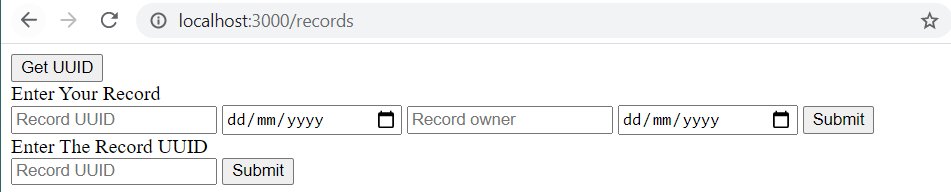
\includegraphics[scale=0.7]{recordsview}
  \caption{Records view}
  \label{fig:recordsview}
\end{figure}

Figure \ref{fig:recordsview} displays the \lstinline{records} view, in this view there is a button to generate a UUID. 
When clicked, this button sends a \lstinline{GET} request to \lstinline{/records/genuuid}, a route that calls the \lstinline{createuuid} function in the controller which returns a UUID to be used in the form. 

The file \lstinline{records.js}, located in the models directory, defines a schema for Records. 
The schema maps to the MongoDB collection and defines the shape of the documents in the collection \cite{noauthor_mongoose_nodate}. 
The file can be found in the appendix \ref{appendix:model}.

As shown in figure \ref{fig:recordsview}, the input boxes for the dates are HTML date pickers, restricting the input to that of a date format. 

\begin{figure}[H]
  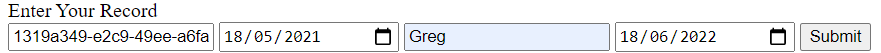
\includegraphics[scale=0.7]{filled}
  \caption{Form filled}
  \label{fig:filled}
\end{figure}

Figure \ref{fig:filled} shows the records form filled with data, ready to be submitted. 
These form values are supplied in a \lstinline{POST} request, to \lstinline{/addrecord}, the route handling the request calls the \lstinline{create()} function which is imported to the routes files from the controller.
The function is called with the parameters for the request and result, enabling the create function in the controller to instantiate a new object based on the \lstinline{Record} schema.
This object's \lstinline{timestamp} and \lstinline{expiration} attributes are parsed using the \lstinline{Date.parse()} function \cite{noauthor_dateparse_nodate}, so that the Date types are replaced by the number of miliseconds since January 1, 1970. 
This simplifies the comparison of dates for checking expiration of immunisation records.
A hash of the UUID is saved to the database and the \lstinline{submit()} function in the controller is called, with the newly created object passed as a parameter. 
As explained previously, the setup required for producing user credentials, registering and enrolling the user is then executed. 
The function then, using the contract that was obtained using the gateway and then network objects, invokes the chaincode. 
A few functions are called, firstly, the \lstinline{InitLedger} function, which sets up some dummy data in the network. 
The function utilises the \lstinline{evaluateTransaction} function provided by the contract API.
The output from this chaincode invocation, as well as the previous function calls, is displayed in figure \ref{fig:init}.

\begin{figure}[H]
  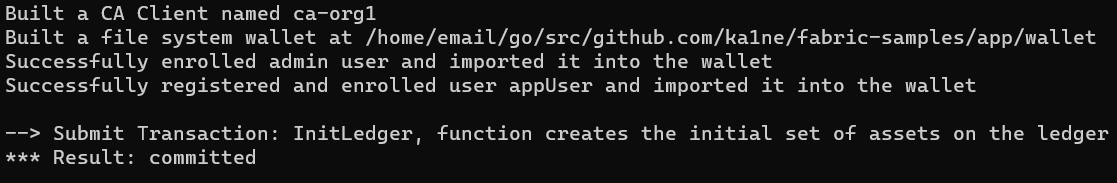
\includegraphics[scale=0.6]{init}
  \caption{Setup and InitLedger output}
  \label{fig:init}
\end{figure}

The chaincode is available in the appendix \ref{appendix:chaincode}. 

After initialisation of the ledger is complete, the \lstinline{GetAllAssets} function is called.
Again, this uses the \lstinline{evaluateTransaction} function supplied by the contract API.  
The function returns all data intialised by the previous function, \lstinline{InitLedger}.
The output can be seen in figure \ref{fig:getall}

\begin{figure}[H]
  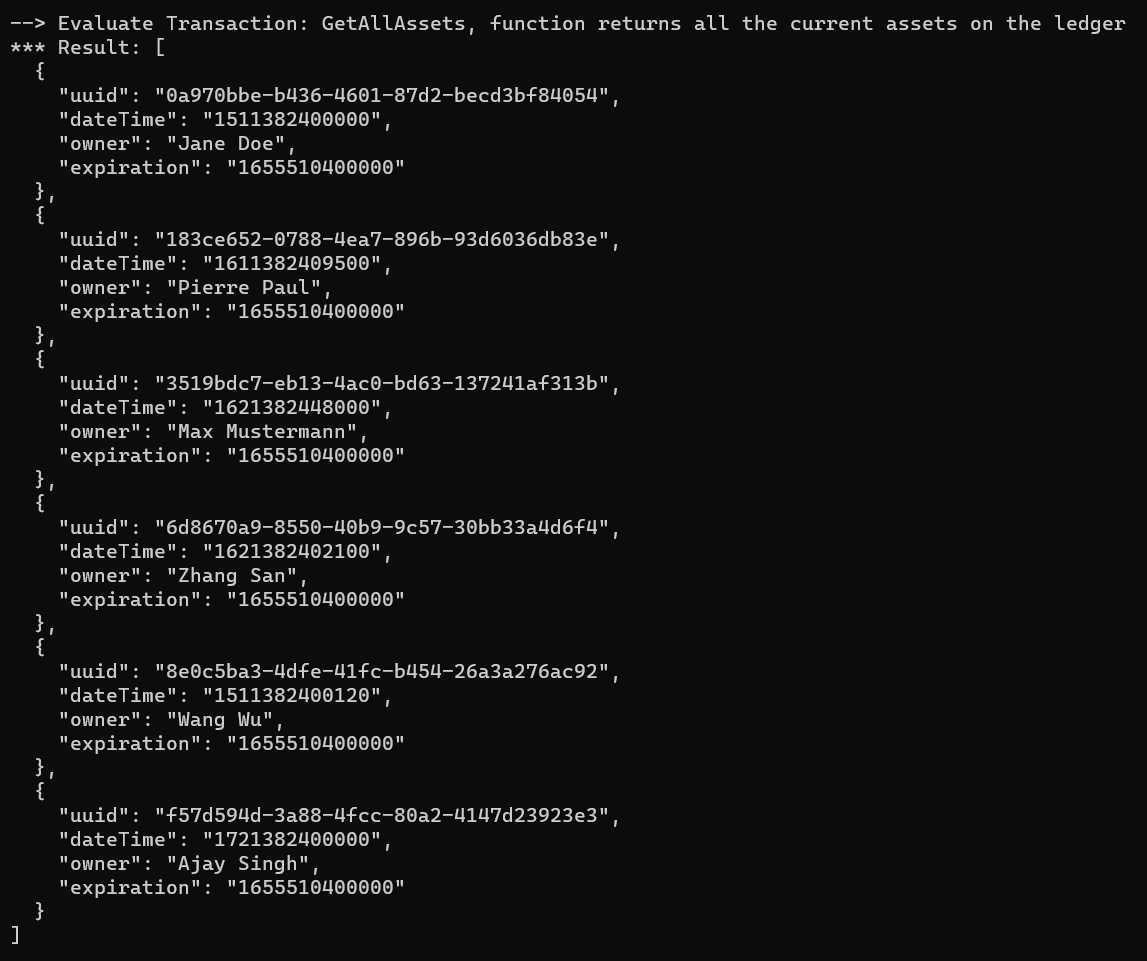
\includegraphics[scale=0.6]{getall}
  \caption{GetAllAssets outut}
  \label{fig:getall}
\end{figure}

Next, the \lstinline{CreateAsset} function is called, with the necessary data from the form in the \lstinline{records} view passed as parameters. 
This time, the \lstinline{submitTransaction} function from the contract API is used. 
This processes commits the transaction, with the newly created asset, to the ledger. 
The output for this function can be seen in figure \ref{fig:submit}.

\begin{figure}[H]
  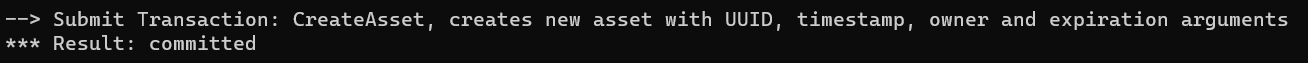
\includegraphics[scale=0.5]{submit}
  \caption{CreateAsset output}
  \label{fig:submit}
\end{figure}

The function \lstinline{ReadAsset} is next to be called, this function takes the record UUID as a parameter. 
This value is used to lookup the corresponding record in the ledger. 
The \lstinline{ReadAsset} function uses the context supplied by the contract API to find the record and returns it to the controller.
The results retrieved are shown in figure \ref{fig:read}.

\begin{figure}[H]
  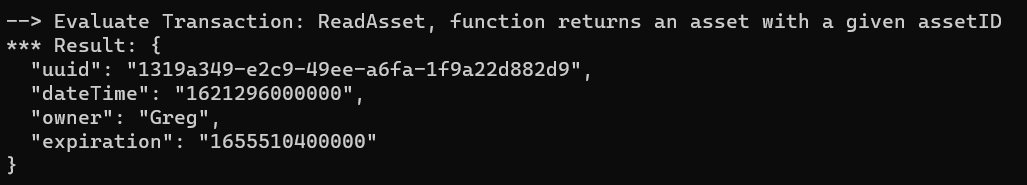
\includegraphics[scale=0.5]{read}
  \caption{ReadAsset output}
  \label{fig:read}
\end{figure}

Following is the call to the \lstinline{AssetExists} function, which checks a record UUID against the ledger to find if the corresponding asset is present. 
A boolean is returned, dependant on if the asset was found. 
The output for this command is shown in figure \ref{fig:exists}. 

\begin{figure}[H]
  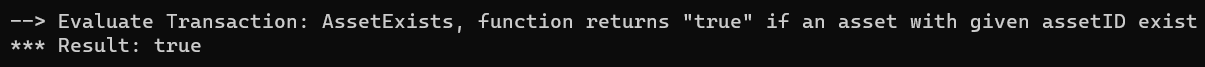
\includegraphics[scale=0.5]{exists}
  \caption{AssetExists output}
  \label{fig:exists}
\end{figure}

Finally, the function \lstinline{AssetValid} is called, this function takes a UUID as an input parameter, finds the relevant asset and unmarshals the JSON representation of the asset. 
Then, the values for \lstinline{timestamp} and \lstinline{expiration} are converted to type \lstinline{Uint64}, compared to check that the timestamp is smaller than the expiration and returns true if so.
This function is the way records are checked for validity, to ensure that the immunisation record has not expired.
The output for this function is shown in figure \ref{fig:valid}.

\begin{figure}[H]
  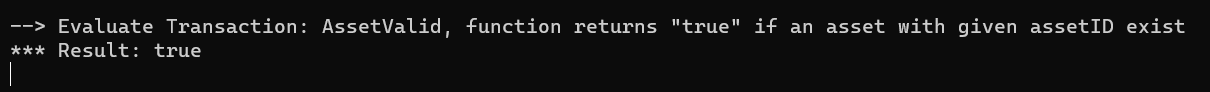
\includegraphics[scale=0.5]{valid}
  \caption{AssetValid output}
  \label{fig:valid}
\end{figure}

Utilising the \lstinline{AssetValid} function from the chaincode is key in verifying records, without the need for the verifier to ever handle the information in the ledger.
Patients with immunisation records in the ledger can provide their UUID for verifiers to enter in the alternative form on the records view. 
For demonstration purposes an existing record, produced by the \lstinline{InitLedger} function shall be used to check the validity of the record. 
The view, with an entered UUID can be seen in figure \ref{fig:validating}.

\begin{figure}[H]
  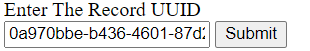
\includegraphics[scale=1]{validating}
  \caption{Record validation form}
  \label{fig:validating}
\end{figure}

On submit of the form, a \lstinline{POST} request is made to \lstinline{/checkrecord} with the data in the request body. 
The route handling this request calls the \lstinline{check} function, imported from the controller.
This function first creates a new \lstinline{Record} object, utilising the schema described previously, using the data from the request body. 
The object is used as a parameter to the \lstinline{find} function, provided by Mongoose \cite{noauthor_mongoose_find}, to check the record is held in the database. 
Next, the \lstinline{checkRecord()} function is called, passing the newly generated \lstinline{Record} object as a parameter. 
A hash of the UUID is stored in the database.
Again, setup is performed via the formerly described sequence of functions for enrolling and registering a user and instantiating a gateway object. 
These credentials are then used to connect to the gateway, enabling access to the underlying network via chaincode invocation. 
The same functions ran previously are again called, the important one being the \lstinline{AssetValid} which looks up the record corresponding to the provided UUID in the ledger, then returns a boolean value showing the validity of the immunisation record. 
A simple comparison is made to check that the \lstinline{timestamp} date is before the \lstinline{expiration} date.
The output generating by this function is displayed in figure \ref{fig:validagain}.

\begin{figure}[H]
  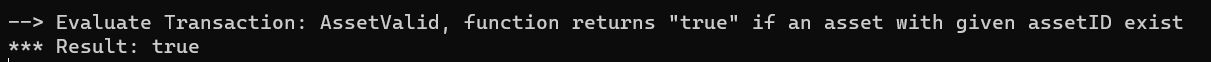
\includegraphics[scale=0.5]{validagain}
  \caption{ValidAsset output}
  \label{fig:validagain}
\end{figure}

To demonstrate the result gained if an expired immunisation record is attempted to be verified, another call to the function is made using a record which is expired. 
The resulting output is available in figure \ref{fig:expired}. As shown in the figure, the function has responded with \lstinline{false} to indicate that the expiration date on the record has been reached.

\begin{figure}[H]
  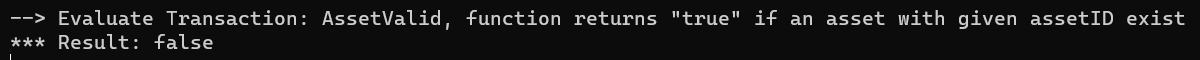
\includegraphics[scale=0.5]{expired}
  \caption{ValidAsset output from an expired contract}
  \label{fig:expired}
\end{figure}

\paragraph{Containerisation}
Code for the files utilised by docker during the containerisation of the web application can be found in the appendix \ref{appendix:containerisation}.
Containersation of the web application running on Node was successful, the files in the appendix can be utilised to compose all necessary services for the web application. 
This includes the MongoDB database. 
However, interaction with the Hyperledger Fabric network was not implemented and so the application is relying on the CLI instead. 
